\documentclass[aspectratio=169,20pt]{beamer}
\geometry{paperwidth=33.87cm, paperheight=19.05cm}

% Update Beamer's internal page dimensions to match
\makeatletter
\beamer@paperwidth=33.87cm
\beamer@paperheight=19.05cm
\makeatother
% =============================================================================
% THEME CONFIGURATION - White background, black text, light grey headings
% =============================================================================
\usetheme{default}
\usecolortheme{default}

% Define colors
\definecolor{headinggrey}{RGB}{240,240,240}
\definecolor{darkgrey}{RGB}{80,80,80}
\definecolor{accentblue}{RGB}{50,100,150}
\definecolor{textblack}{RGB}{0,0,0}

% Set beamer colors
\setbeamercolor{background canvas}{bg=white}
\setbeamercolor{normal text}{fg=textblack}
\setbeamercolor{frametitle}{bg=headinggrey,fg=textblack}
\setbeamercolor{title}{fg=textblack}
\setbeamercolor{subtitle}{fg=darkgrey}
\setbeamercolor{author}{fg=darkgrey}
\setbeamercolor{date}{fg=darkgrey}
\setbeamercolor{institute}{fg=darkgrey}
\setbeamercolor{item}{fg=accentblue}
\setbeamercolor{block title}{bg=headinggrey,fg=textblack}
\setbeamercolor{block body}{bg=white,fg=textblack}
\setbeamercolor{block title alerted}{bg=headinggrey,fg=red}
\setbeamercolor{block title example}{bg=headinggrey,fg=accentblue}

% Remove navigation symbols
\setbeamertemplate{navigation symbols}{}

\setbeamertemplate{footline}{%
	\hfill%
	\usebeamercolor[fg]{page number in head/foot}%
	\usebeamerfont{page number in head/foot}%
	\insertframenumber{}\hspace*{2ex}%
	\vskip2pt%
}
% ------------------------------------------------------------------------------

% Frame title template with light grey box
\setbeamertemplate{frametitle}{
	\vspace{0.2cm}
	\begin{beamercolorbox}[wd=\paperwidth,ht=0.8cm,dp=0.3cm]{frametitle}
		\hspace{0.5cm}\usebeamerfont{frametitle}\insertframetitle
	\end{beamercolorbox}
	\vspace{0.2cm}
}

% Packages
\usepackage{amsmath,amssymb,amsthm}
\usepackage{mathtools}
\usepackage{graphicx}
\usepackage{booktabs}
\usepackage{siunitx}
\usepackage{tikz}
\usetikzlibrary{arrows.meta,positioning,calc,shapes,decorations.pathmorphing,fit,backgrounds}
\usepackage{bm}
\usepackage{xcolor}
\usepackage{multicol}
\usepackage{multirow}
\usepackage{pgfplots}
\pgfplotsset{compat=1.18}

% Custom commands
\newcommand{\vect}[1]{\mathbf{#1}}
\newcommand{\mat}[1]{\mathbf{#1}}
\newcommand{\spike}{\text{spike}}
\newcommand{\LIF}{\text{LIF}}
\newcommand{\STDP}{\text{STDP}}
\newcommand{\SNR}{\text{SNR}}
\newcommand{\ERB}{\text{ERB}}


% Title info
\title[Neuromorphic Cochlea]{\textbf{Neuromorphic Cochlea and SNN-Based\\Pitch Classification}}
\subtitle{From Preprocessing to ``Absolute Pitch'' Models}
%\author[Georgii Kormakov]{Neuromorphic Computing Course Project}
%\institute[]{Skoltech}
%\date{May 2026}

% Path for figures
\graphicspath{{./imgs}}

\begin{document}

% =============================================================================
% TITLE SLIDE
% =============================================================================
{
\setbeamertemplate{frametitle}{}
\begin{frame}[noframenumbering, plain] 
\vspace{1.5cm}
\begin{center}
    {\LARGE\textbf{Neuromorphic Cochlea and SNN-Based}}\\[0.3cm]
    {\LARGE\textbf{Pitch Classification}}\\[0.8cm]
    %{\large Final Project Results}\\[0.3cm]
    {\normalsize From Preprocessing to ``Absolute Pitch'' Models}\\[1.5cm]
    %{\normalsize Neuromorphic Computing Course Project}\\[0.3cm]
    %{\small Skoltech}\\[0.5cm]
    %{\small May 2026}
\end{center}
\end{frame}
}
\setcounter{framenumber}{12}
% =============================================================================
% OUTLINE
% =============================================================================
% \begin{frame}{Presentation Overview}
% \tableofcontents
% \end{frame}

% =============================================================================
% SECTION 1: INTRODUCTION
% =============================================================================
\section{Introduction}

\begin{frame}{Project Goals and Timeline}
\begin{block}{Research Objective}
Develop a bio-inspired spiking neural network for robust musical pitch classification.
%, comparing custom preprocessing (``handy'') against library implementation (``spikify'').
\end{block}

\vfill
\textbf{Experimental Timeline:}
\begin{enumerate}
    \item Implemented custom auditory preprocessing pipeline
    \item Discovered and fixed ERB scaling  ($\times 1000$ error)
    \item 3-tone classification (C4, A4, A5) -- 100\% accuracy
    \item Full 88-key piano classification -- 58\% accuracy
    \item STDP-based unsupervised learning comparison
\end{enumerate}

\vfill
\textbf{Key Finding:} Handy preprocessing shows superior noise robustness despite slower training convergence.
\end{frame}

% =============================================================================
% SECTION 2: MATHEMATICAL BACKGROUND
% =============================================================================
\section{Mathematical Background}

\begin{frame}{ERB Scale: Three Implementations}
\begin{block}{Equivalent Rectangular Bandwidth (ERB) Scale}
Perceptual frequency scale modeling human auditory filter bandwidths.
\end{block}

\vspace{0.3cm}
\begin{columns}
\begin{column}{0.48\textwidth}
\textbf{Linear ERB} (Glasberg \& Moore, 1990):
\begin{equation*}
\ERB(F) = 24.7 \cdot (4.37F + 1) \quad [\text{Hz}]
\end{equation*}
\begin{equation*}
\text{ERBS}(f) = 21.4 \log_{10}(1 + 4.37f) \quad [\text{kHz}]
\end{equation*}

\vspace{0.2cm}
\textbf{Quadratic ERB}:
\begin{equation*}
\ERB(F) = 6.23F^2 + 93.39F + 28.52
\end{equation*}
\begin{equation*}
	\text{ERBS}(f) = 11.17 \cdot \ln\left(\frac{f+0.312}{f+14.675}\right) + 43.0
\end{equation*}
\end{column}

\begin{column}{0.48\textwidth}
\textbf{Voicebox ERB}:
\begin{equation*}
\text{ERBS}(f) = a\ln\left(h - \frac{k}{f+c}\right)
\end{equation*}
where $a = 11.17$, $h = 47.07$, $k = 676170$, $c = 14678$

\vspace{0.3cm}
\textbf{Inverse Mapping:}
\begin{equation*}
f = \frac{k}{h - \exp(\text{ERBS}/a)} - c
\end{equation*}
\end{column}
\end{columns}

\vspace{0.3cm}
\begin{center}
\textit{Critical Bug: Quadratic and Linear ERB had wrong scaling factor ($\times 1000$) at return!}
\end{center}
\end{frame}

\begin{frame}{ERB Scale: Valid ranges}
\begin{columns}
	\begin{column}{\textwidth}
		\centering
		
\includegraphics[width=\textwidth]{erb_comparison.pdf}
	\end{column}
\end{columns}
\end{frame}

\begin{frame}{Gammatone Filterbank}
\begin{block}{Filter Impulse Response}
Time-domain FIR approximation of cochlear filtering:
\begin{equation}
h_i(t) = t^{n-1} e^{-2\pi b_i t} \cos(2\pi f_i t + \phi), \quad n=4
\end{equation}
where $f_i$ are center frequencies spaced on ERB scale, $b_i = 1.019 \cdot \ERB(f_i)$
\end{block}

\vspace{0.01cm}
\textbf{Filterbank Processing:}
\begin{equation}
x_i(t) = (x * h_i)(t), \quad i = 1, \ldots, N_{\text{chan}}
\end{equation}

\vspace{-0.1cm}
\begin{columns}
\begin{column}{0.48\textwidth}
\textbf{Parameters:}
\begin{itemize}
    \item $N_{\text{chan}} = 50$ channels
    \item $f_{\text{low}} = 100$ Hz
    \item $f_{\text{high}} = 6500$ Hz
    \item IR duration: 50 ms
\end{itemize}
\end{column}
\begin{column}{0.48\textwidth}
\textbf{Implementation:}
\begin{itemize}
    \item FFT convolution for speed
    \item Normalized impulse response
    \item Mode: `same' for alignment
\end{itemize}
\end{column}
\end{columns}
\end{frame}

\begin{frame}{Inner Hair Cell and Spike Generation}
\begin{block}{Inner Hair Cell (IHC) Model}
Soft half-wave rectification followed by power-law compression:
\begin{equation}
r_i(t) = \max(0, x_i(t))^{0.7}
\end{equation}
\end{block}

\vspace{-0.5cm}
\begin{block}{Poisson Spike Generation}
Inhomogeneous Poisson process with rate proportional to IHC output:
\begin{equation}
P(\text{spike in } [t, t+dt)) = \lambda_i(t) \cdot dt = \gamma \cdot \frac{r_i(t)}{r_{\max}} \cdot \max_{\text{rate}} \cdot dt
\end{equation}
\end{block}

\vspace{-0.4cm}
\textbf{Relative Rate Logic:}
\begin{itemize}
    \item Global maximum across all channels: $r_{\max} = \max_{i,t} r_i(t)$
    \item Preserves relative loudness between channels
    \item High-energy channels fire at $\max_{\text{rate}} = 800 \text{ Hz}$, low-energy near 0 Hz
\end{itemize}
\end{frame}

\begin{frame}{Pipeline Architecture}
	\begin{center}
		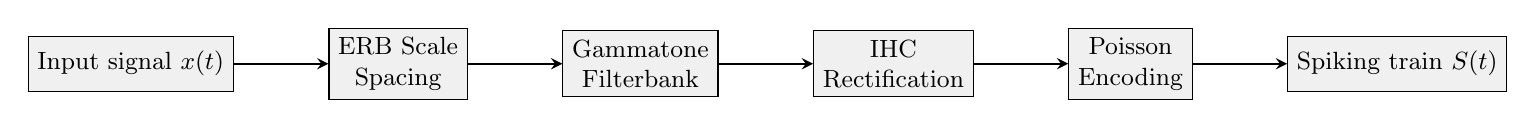
\begin{tikzpicture}[
			node distance=1.2cm,
			box/.style={rectangle, draw=black, fill=headinggrey, minimum width=0.7cm, minimum height=0.7cm, align=center, font=\small},
			arrow/.style={->, >=stealth, thick}
			]
			% Nodes
			\node[box] (input) {Input signal $x(t)$};
			\node[box, right=of input] (erb) {ERB Scale\\Spacing};
			\node[box, right=of erb] (gamma) {Gammatone\\Filterbank};
			\node[box, right=of gamma] (ihc) {IHC\\Rectification};
			\node[box, right=of ihc] (poisson) {Poisson\\Encoding};
			\node[box, right=of poisson] (output) {Spiking train $S(t)$};
			
			% Arrows
			\draw[arrow] (input) -- (erb);
			\draw[arrow] (erb) -- (gamma);
			\draw[arrow] (gamma) -- (ihc);
			\draw[arrow] (ihc) -- (poisson);
			\draw[arrow] (poisson) -- (output);
		\end{tikzpicture}
	\end{center}
	
	\vspace{0.4cm}
	\textbf{Two Implementations Compared:}
	\begin{columns}
		\begin{column}{0.48\textwidth}
			\textbf{``Handy'' (Custom):}
			\begin{itemize}
				\item Custom ERB implementations
				\item Manual gammatone filters
				\item Relative threshold Poisson
				\item Global/max normalization
			\end{itemize}
		\end{column}
		\begin{column}{0.48\textwidth}
			\textbf{``Spikify'' (Library):}
			\begin{itemize}
				\item Built-in ERB spacing
				\item Optimized filterbank
				\item Standard Poisson encoder
				\item Channel-wise processing
			\end{itemize}
		\end{column}
	\end{columns}
\end{frame}

\begin{frame}{The ERB Scaling Bug and Fix}
	\begin{alertblock}{Bug Discovery}
		Quadratic and Linear ERB scales had incorrect scaling at return:
		\texttt{return value * 1000} instead of correct frequency in Hz.
	\end{alertblock}
	
	\vspace{0.cm}
	\textbf{Impact on Spike Generation:}
	\begin{itemize}
		\item Center frequencies computed incorrectly
		\item Filterbank channels misaligned with input tones
		\item Spike patterns had poor phase-locking
		\item Classification accuracy degraded significantly
	\end{itemize}
	
	\vspace{0.cm}
	\textbf{After Fix:}
	\begin{itemize}
		\item Correct center frequency placement
		\item Improved phase-locking to stimulus period
		\item Clearer frequency-specific channel activation
		\item 100\% accuracy on 3-tone classification
	\end{itemize}

\end{frame}

\begin{frame}{The ERB Scaling Bug and Fix}
	\begin{columns}
		\centering
		\begin{column}{0.48\textwidth}
			\centering
			\textbf{Handy before}
			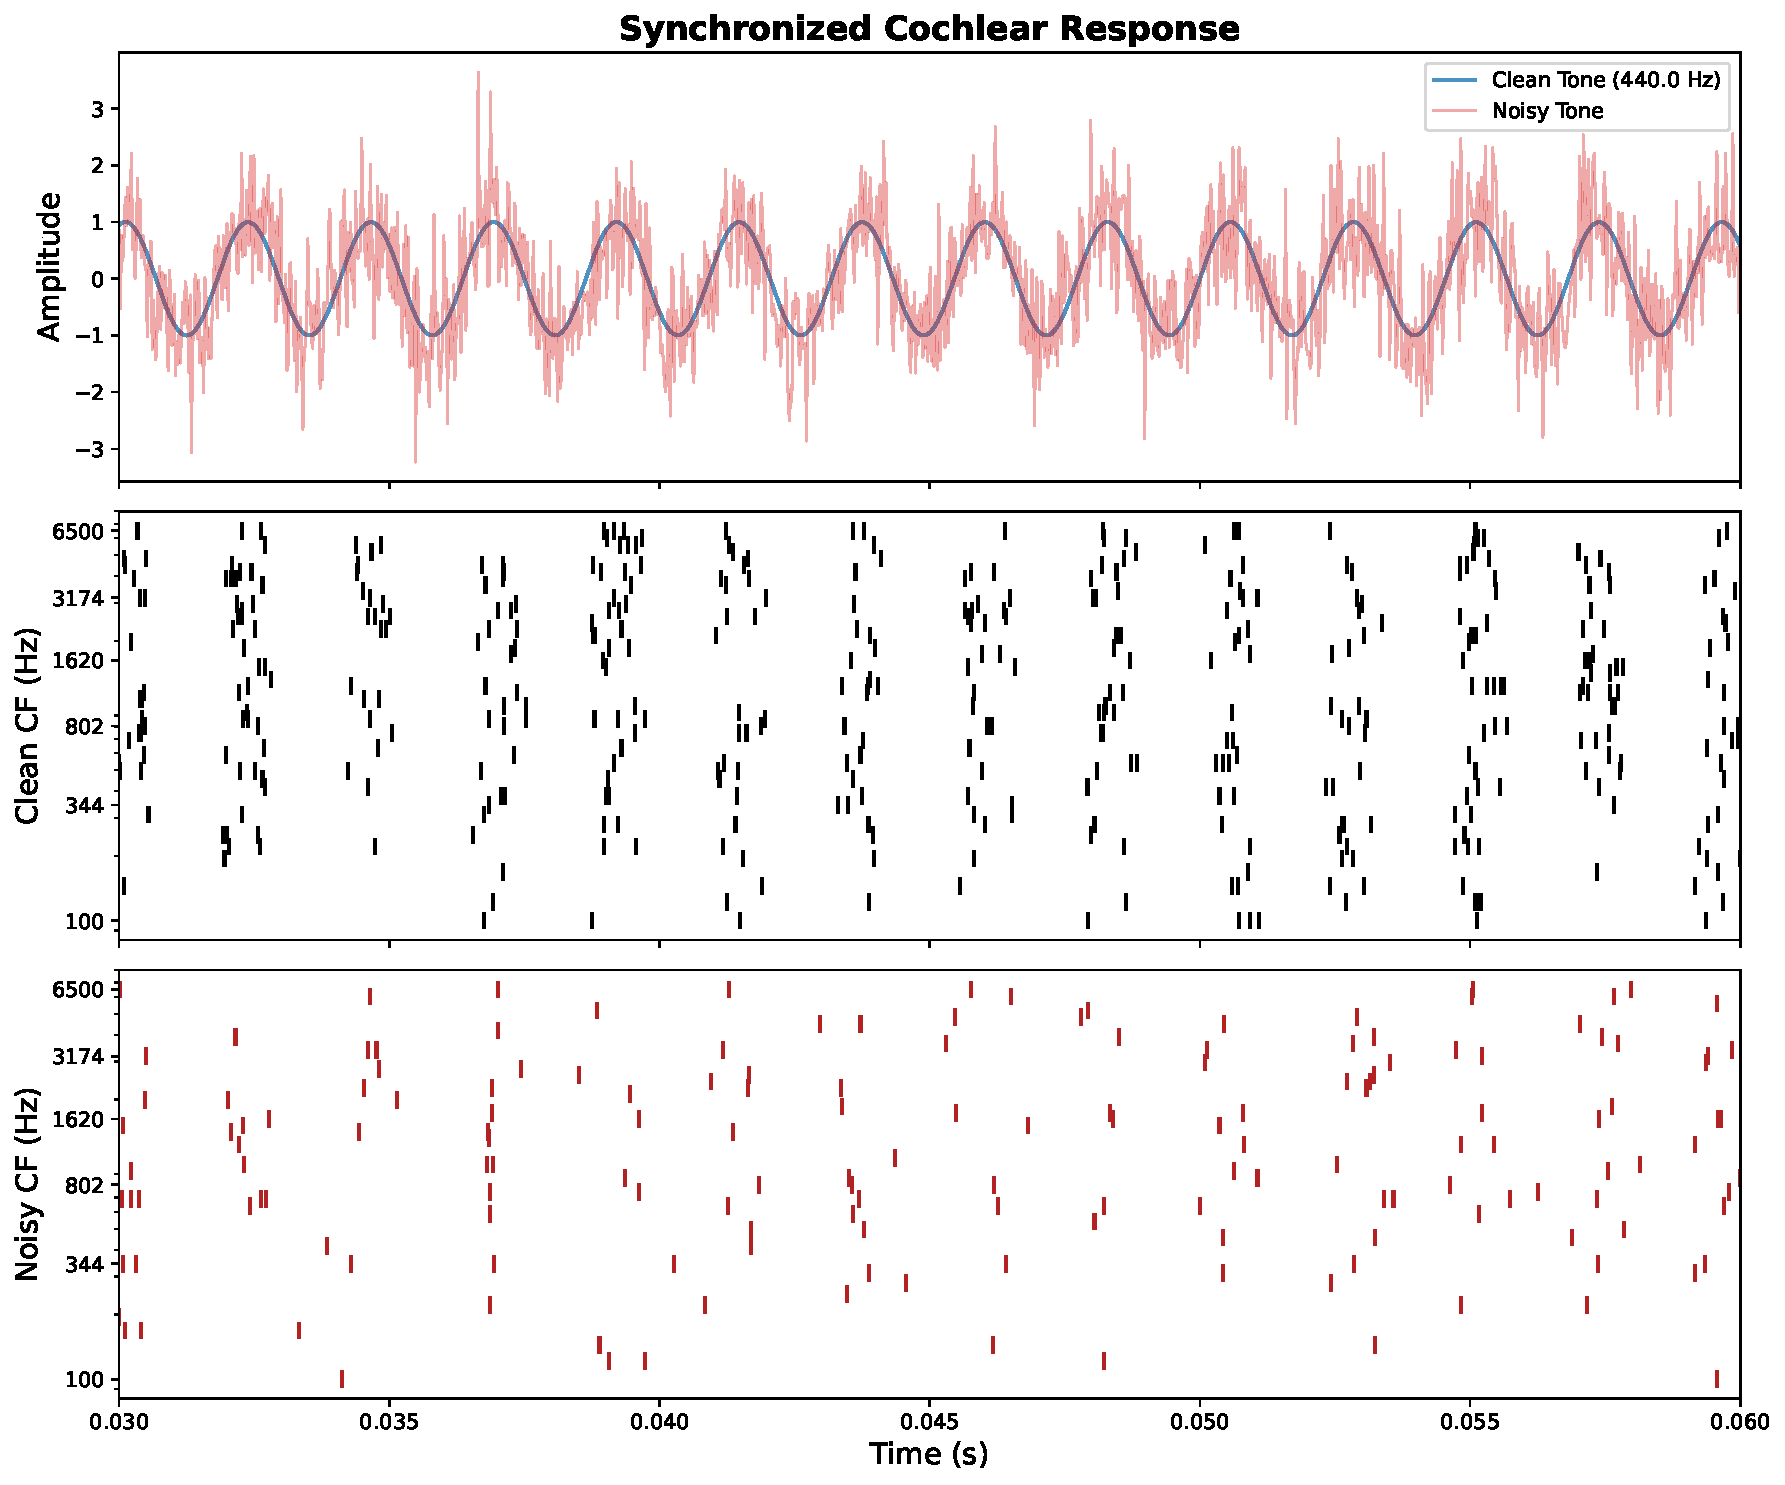
\includegraphics[width=\textwidth]{filterbank_freq440.0_handy.pdf}
		\end{column}
		\begin{column}{0.48\textwidth}
			\centering
			\textbf{Handy after}
			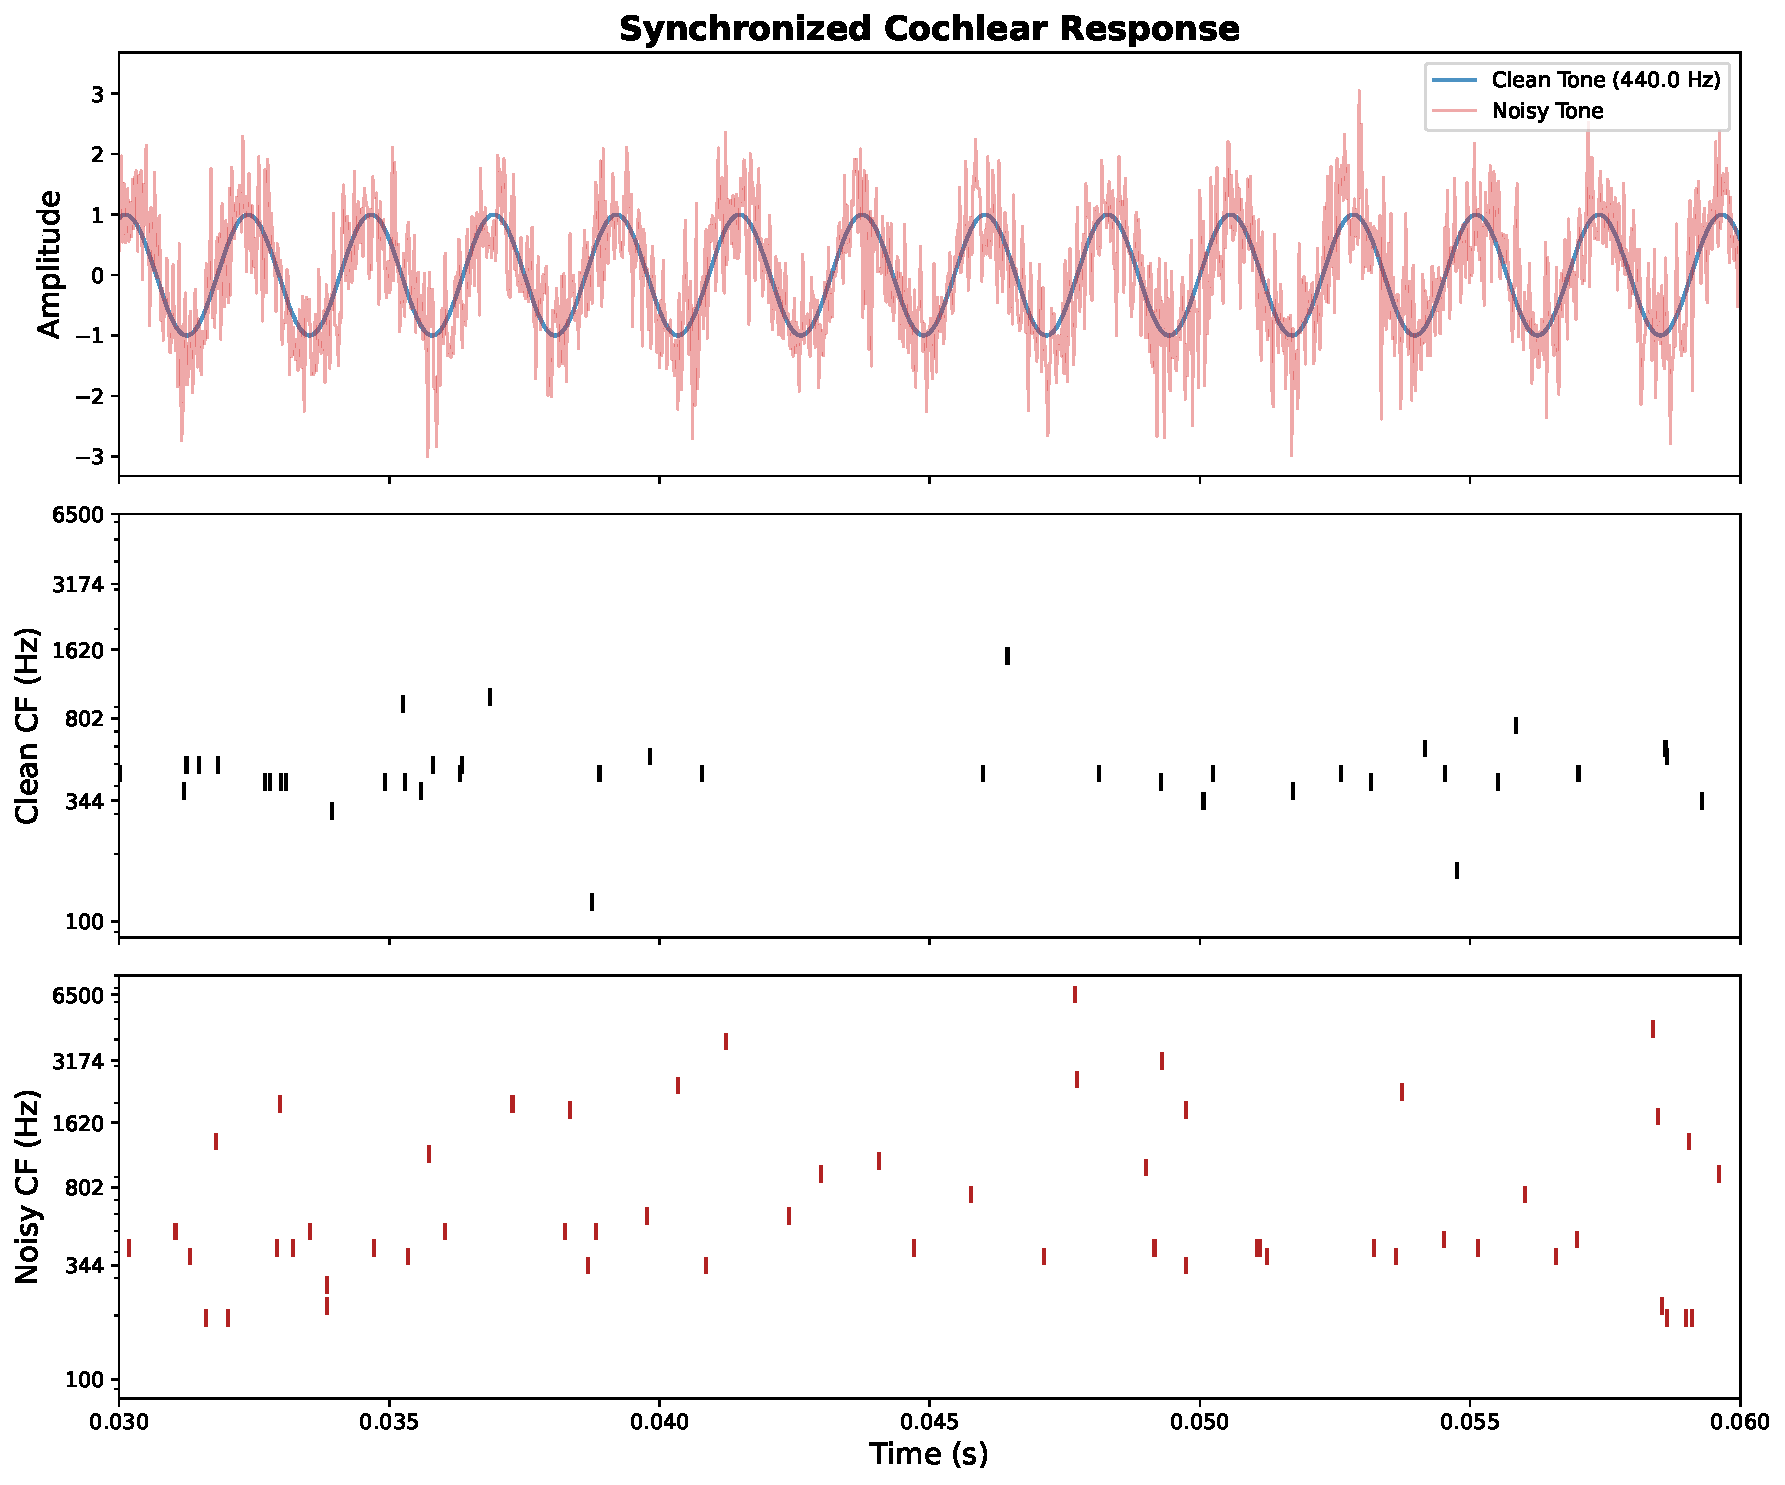
\includegraphics[width=\textwidth]{filterbank_freq440.0_handy_fixed.pdf}
		\end{column}
	\end{columns}
\end{frame}

\begin{frame}{The ERB Scaling Handy vs Spikify}
	\begin{columns}
		\centering
		\begin{column}{0.48\textwidth}
			\centering
			\textbf{Handy}
			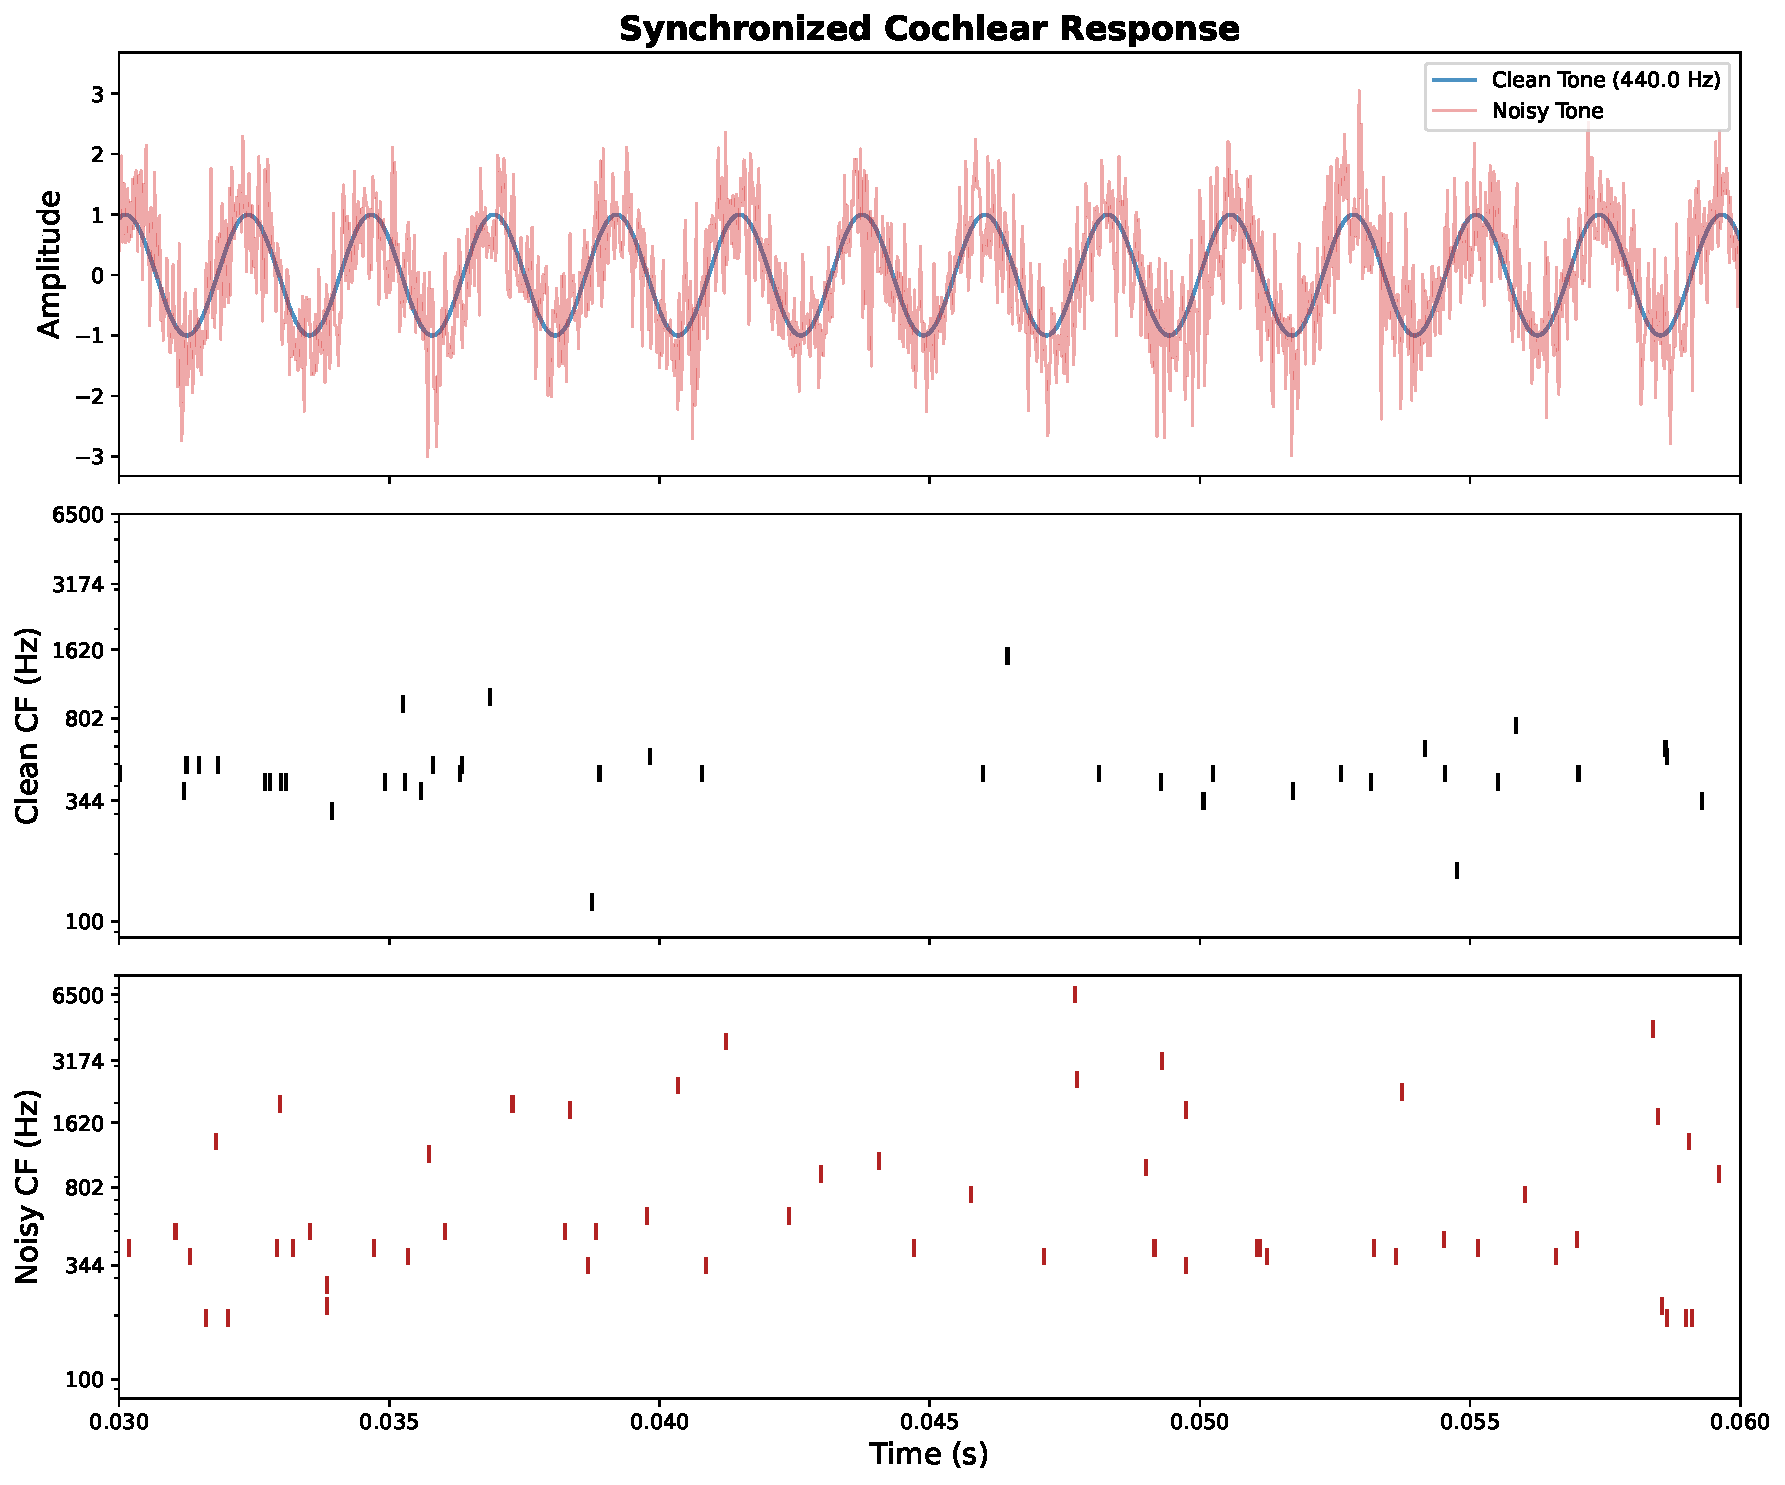
\includegraphics[width=\textwidth]{filterbank_freq440.0_handy_fixed.pdf}
		\end{column}
		\begin{column}{0.48\textwidth}
			\centering
			\textbf{Spikify}
			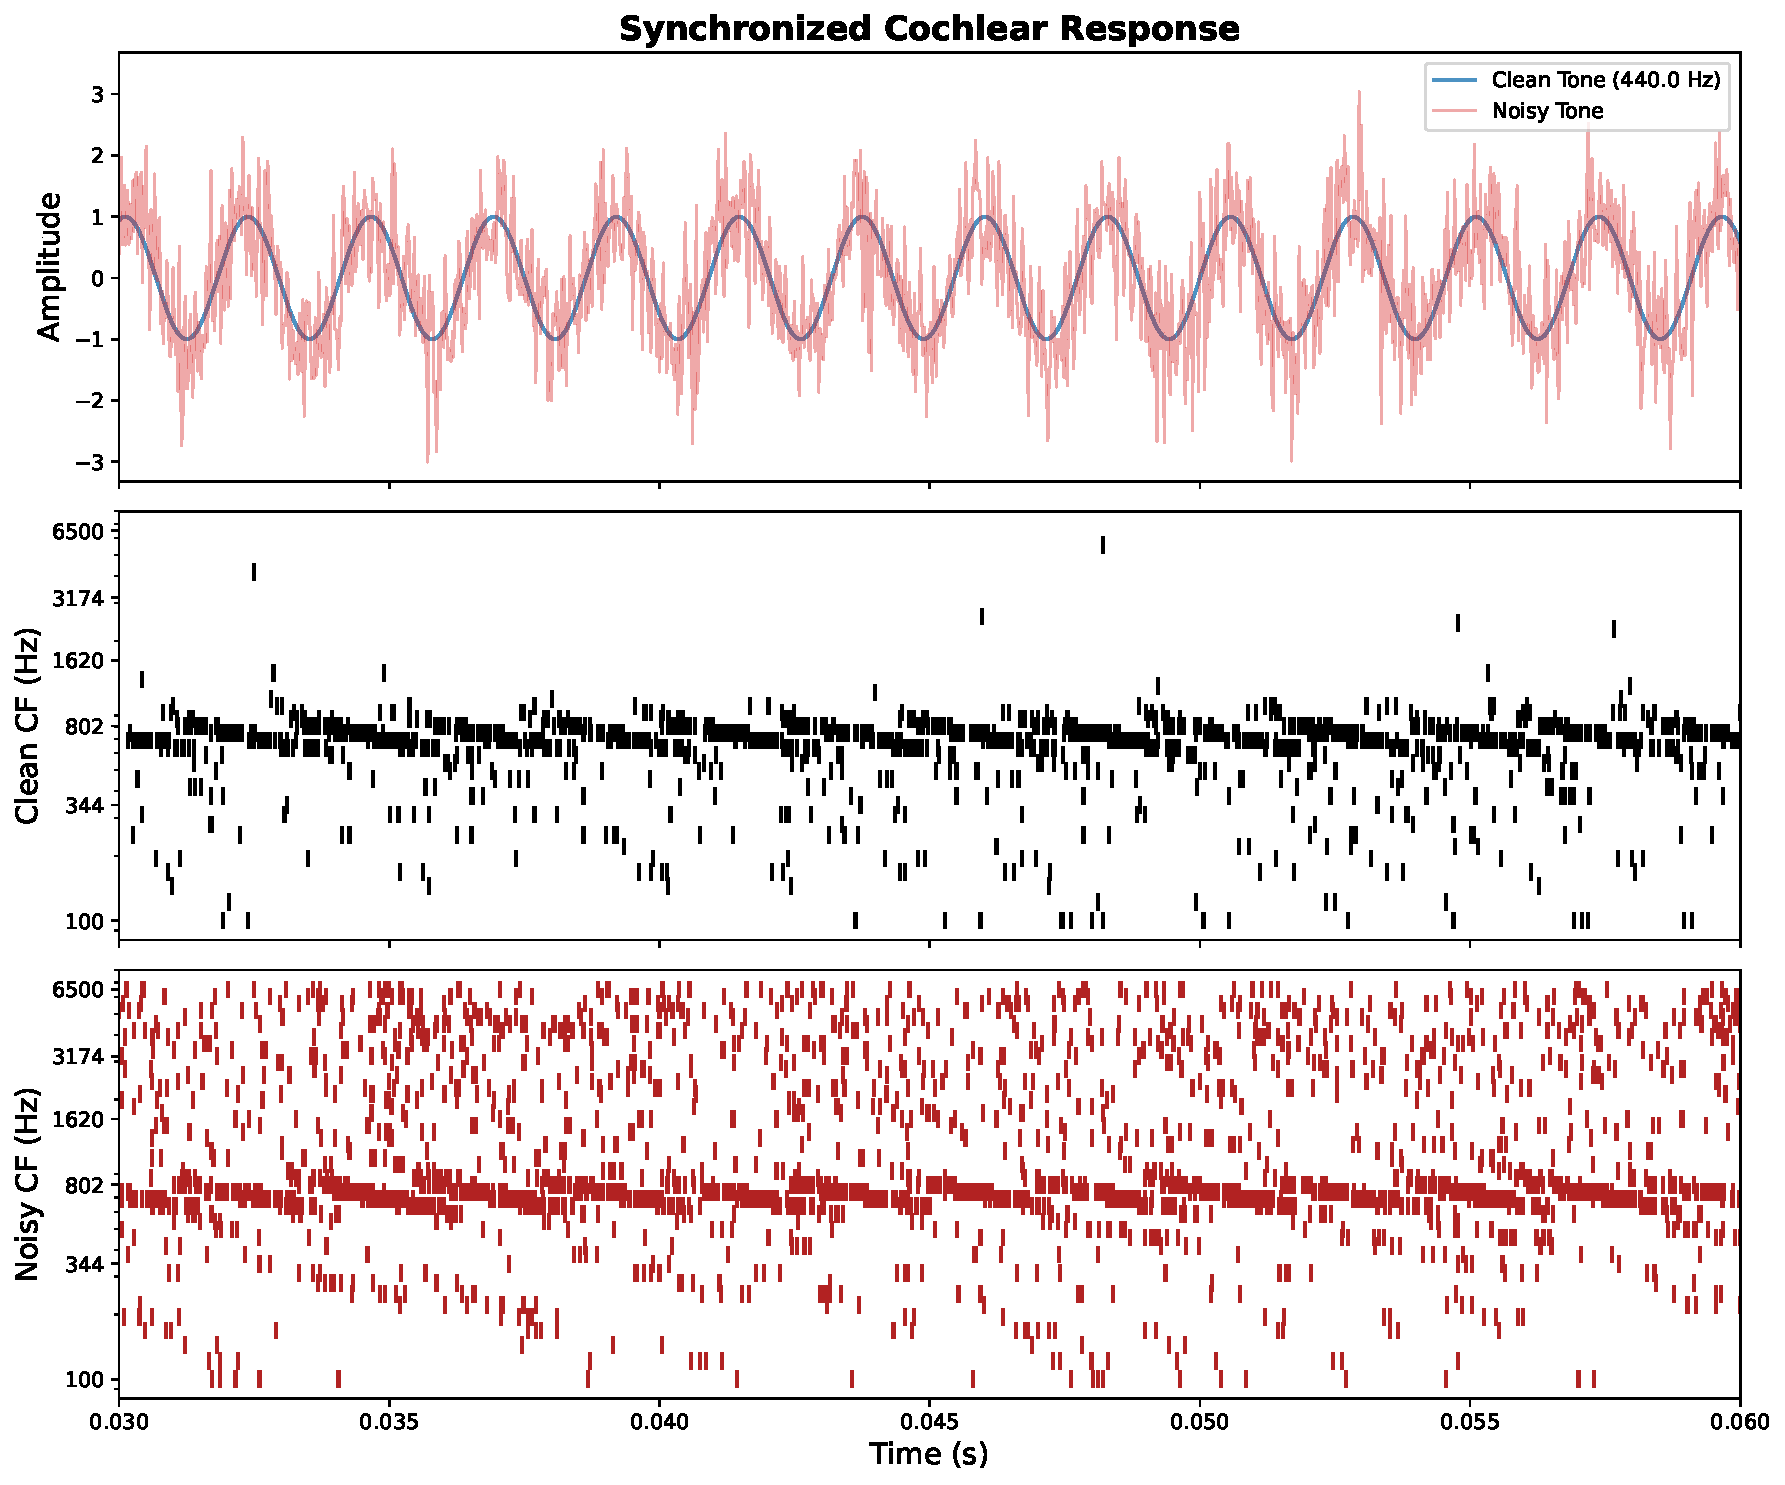
\includegraphics[width=\textwidth]{filterbank_freq440.0_library.pdf}
		\end{column}
	\end{columns}
\end{frame}


\begin{frame}{SNN Architecture: LIF Neuron Dynamics}
\begin{block}{Leaky Integrate-and-Fire (LIF) Model}
\begin{equation}
\tau_m \frac{dV_j}{dt} = -(V_j - V_{\text{rest}}) + R \sum_i w_{ij} s_i(t)
\end{equation}
\begin{equation}
V_j \geq V_{\text{th}} \Rightarrow \text{spike } s_j = 1, \quad V_j \leftarrow V_{\text{reset}}
\end{equation}
\end{block}

\vfill
\textbf{Supervised SNN Architecture (PitchSNN):}
\begin{itemize}
    \item \textbf{Input:} 50 channels (cochlear filters); \textbf{Output:} 3 or 88 LIF neurons;
    \item \textbf{Hidden:} 100 LIF neurons ($\beta = 0.9$)
    \item \textbf{Surrogate gradient:} Fast sigmoid (slope = 25)
\end{itemize}

\vfill
\textbf{Training:} Cross-entropy loss on time-averaged membrane potentials:
\begin{equation}
\mathcal{L} = \text{CE}\left(\frac{1}{T}\sum_{t=1}^{T} \vect{V}_{\text{out}}(t), \; y_{\text{target}}\right)
\end{equation}
\end{frame}

\begin{frame}{3 notes Dataset and Experimental Setup}
	\textbf{Dataset Generation:}
	\begin{itemize}
		\item \textbf{Tones:} C4 (261.63 Hz), A4 (440 Hz), A5 (880 Hz)
		\item \textbf{Duration:} 100 ms pure sine waves
		\item \textbf{Sampling rate:} 44.1 kHz
		\item \textbf{Samples per class:} 60 (training)
		\item \textbf{SNR variance:} Random 10-30 dB for robustness
	\end{itemize}
	
	\vspace{0.cm}
	\textbf{Model Configuration:}
	\begin{itemize}
		\item Input: 50 cochlear channels
		\item Hidden: 100 LIF neurons
		\item Output: 3 classes
		\item Optimizer: Adam (lr = 0.005); Epochs: 20; Batch size: 16
	\end{itemize}
	
	\vspace{0.3cm}
	\begin{block}{Result}
		\textbf{100\% training accuracy} achieved after preprocessing fix for both handy and spikify.
	\end{block}
\end{frame}

\begin{frame}{Noise Robustness Analysis}
	\begin{block}{Evaluation Protocol}
		Test accuracy at progressively worse SNR levels: 20, 10, 5, 0, -5, -10 dB
	\end{block}
	
	\vspace{0.cm}
	\begin{columns}
		\centering
		\begin{column}{0.48\textwidth}
			\centering
			\textbf{Key Finding:}
			\begin{itemize}
				\item \textbf{Handy preprocessing:} Stable training, maintains performance at negative dB
				\item \textbf{Spikify preprocessing:} Faster training accuracy increase, unstable at low SNR
			\end{itemize}
		\end{column}
		\begin{column}{0.48\textwidth}
			\centering
			\textbf{Spikify noise robustness}
			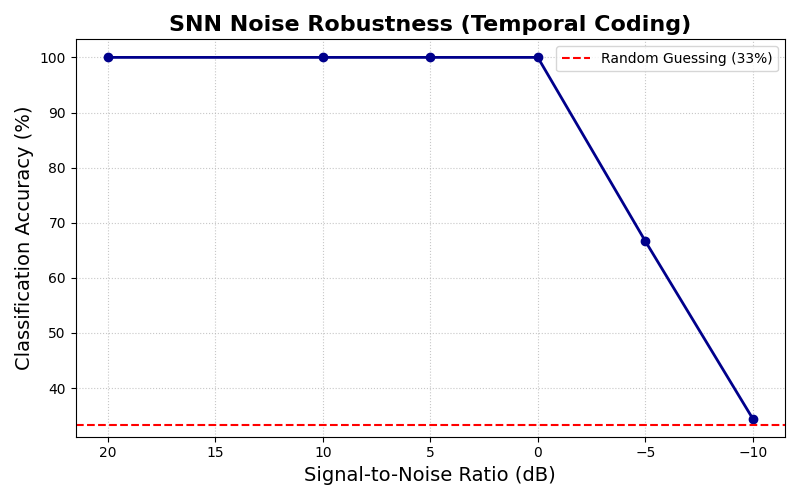
\includegraphics[width=\textwidth]{noise_robustness.png}
		\end{column}
	\end{columns}	
	\vspace{0.3cm}
	\begin{center}
	\end{center}

\end{frame}

\begin{frame}{Full Piano Dataset Generation}
	\textbf{Piano Range:} A0 (27.5 Hz) to C8 (4186.01 Hz)
	
	\vspace{0.3cm}
	\textbf{Frequency Calculation:}
	\begin{equation}
		f_k = f_{A0} \cdot 2^{k/12} = 27.5 \cdot 2^{k/12}, \quad k = 0, 1, \ldots, 87
	\end{equation}
	
	\vspace{0.3cm}
	\textbf{Dataset Parameters:}
	\begin{itemize}
		\item 88 classes (full piano keyboard)
		\item 50 samples per class
		\item Train/test split: 80/20
		\item Total samples: 4,400
		\item Temporal binning: 1 ms (100 time steps)
	\end{itemize}
	
	\vspace{0.3cm}
	\textbf{Adaptive Filterbank:}
	Automatically adjusts $f_{\text{low}}$ and $f_{\text{high}}$ to cover full piano range:
	\begin{equation}
		f_{\text{low}} = \min(100, 27.5), \quad f_{\text{high}} = \max(6500, 4186)
	\end{equation}
\end{frame}

% =============================================================================
% SECTION 5: EXPERIMENT 2 - 88-KEY PIANO CLASSIFICATION
% =============================================================================
\section{Experiment 2: 88-Key Piano Classification}



\begin{frame}{88-Key Piano Training Results: Accuracy Curves}
\begin{columns}
\begin{column}{0.48\textwidth}
\centering
\textbf{Handy Preprocessing}
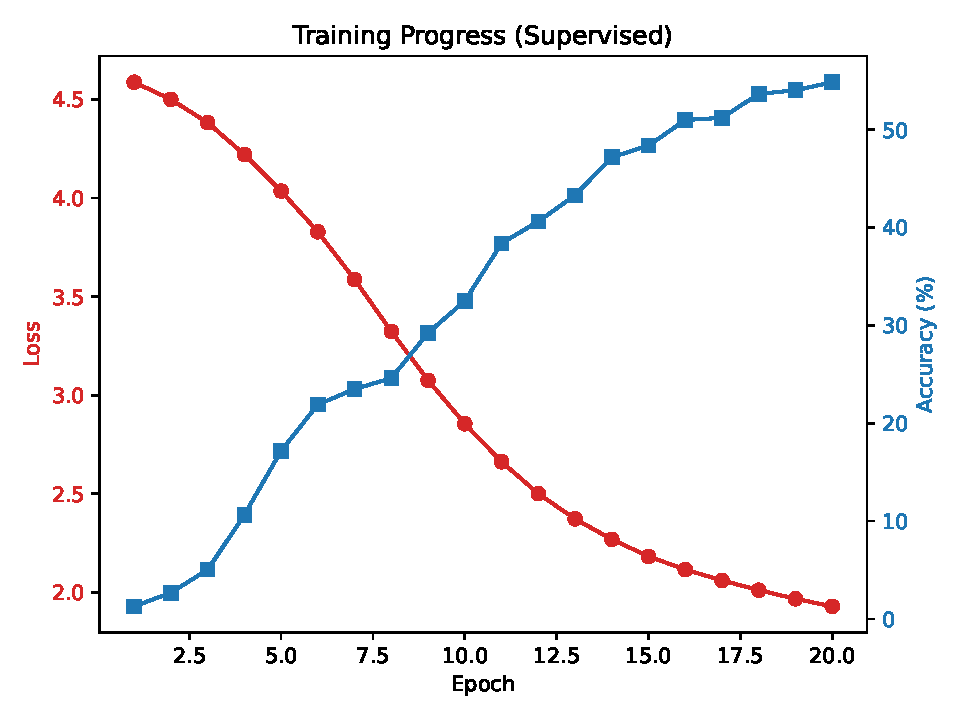
\includegraphics[width=\textwidth]{training_curves_piano88_handy.pdf}

\vspace{-0.2cm}
\begin{itemize}
    \item Slower convergence
    \item More stable training
    \item Final: $\sim$58\% accuracy
\end{itemize}
\end{column}
\begin{column}{0.48\textwidth}
\centering
\textbf{Spikify Preprocessing}
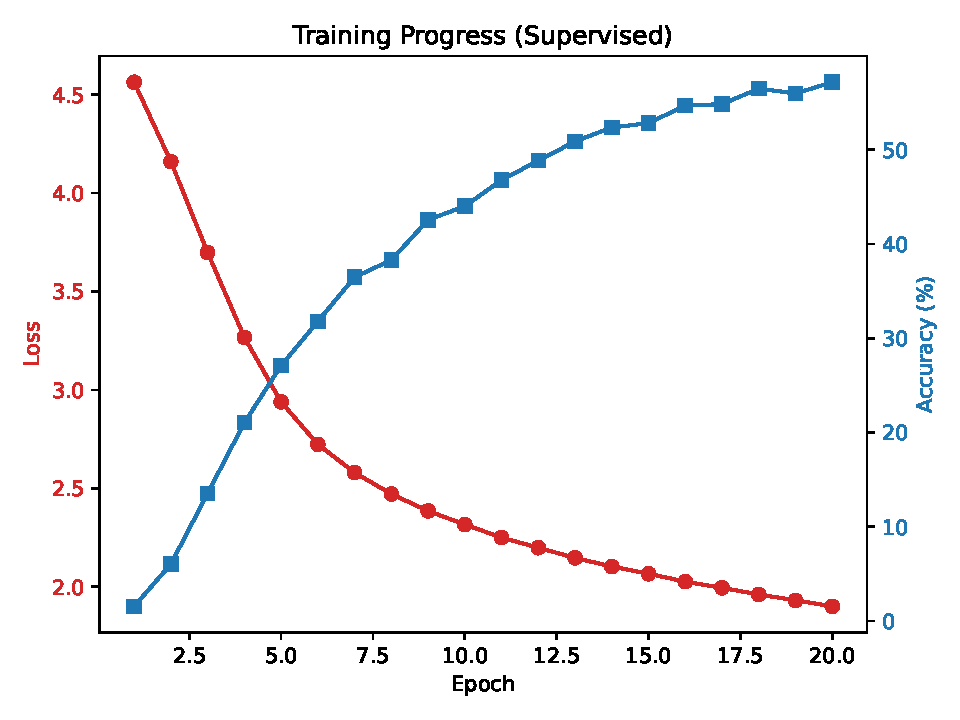
\includegraphics[width=\textwidth]{training_curves_piano88_spikify.pdf}

\vspace{-0.2cm}
\begin{itemize}
    \item Faster initial learning
    \item Higher variance
    \item Final: $\sim$58\% accuracy
\end{itemize}
\end{column}
\end{columns}
\end{frame}

\begin{frame}{88-Key Piano Confusion Matrix Analysis: Error Patterns}
\begin{columns}
\begin{column}{0.48\textwidth}
\centering
\textbf{Handy Preprocessing}
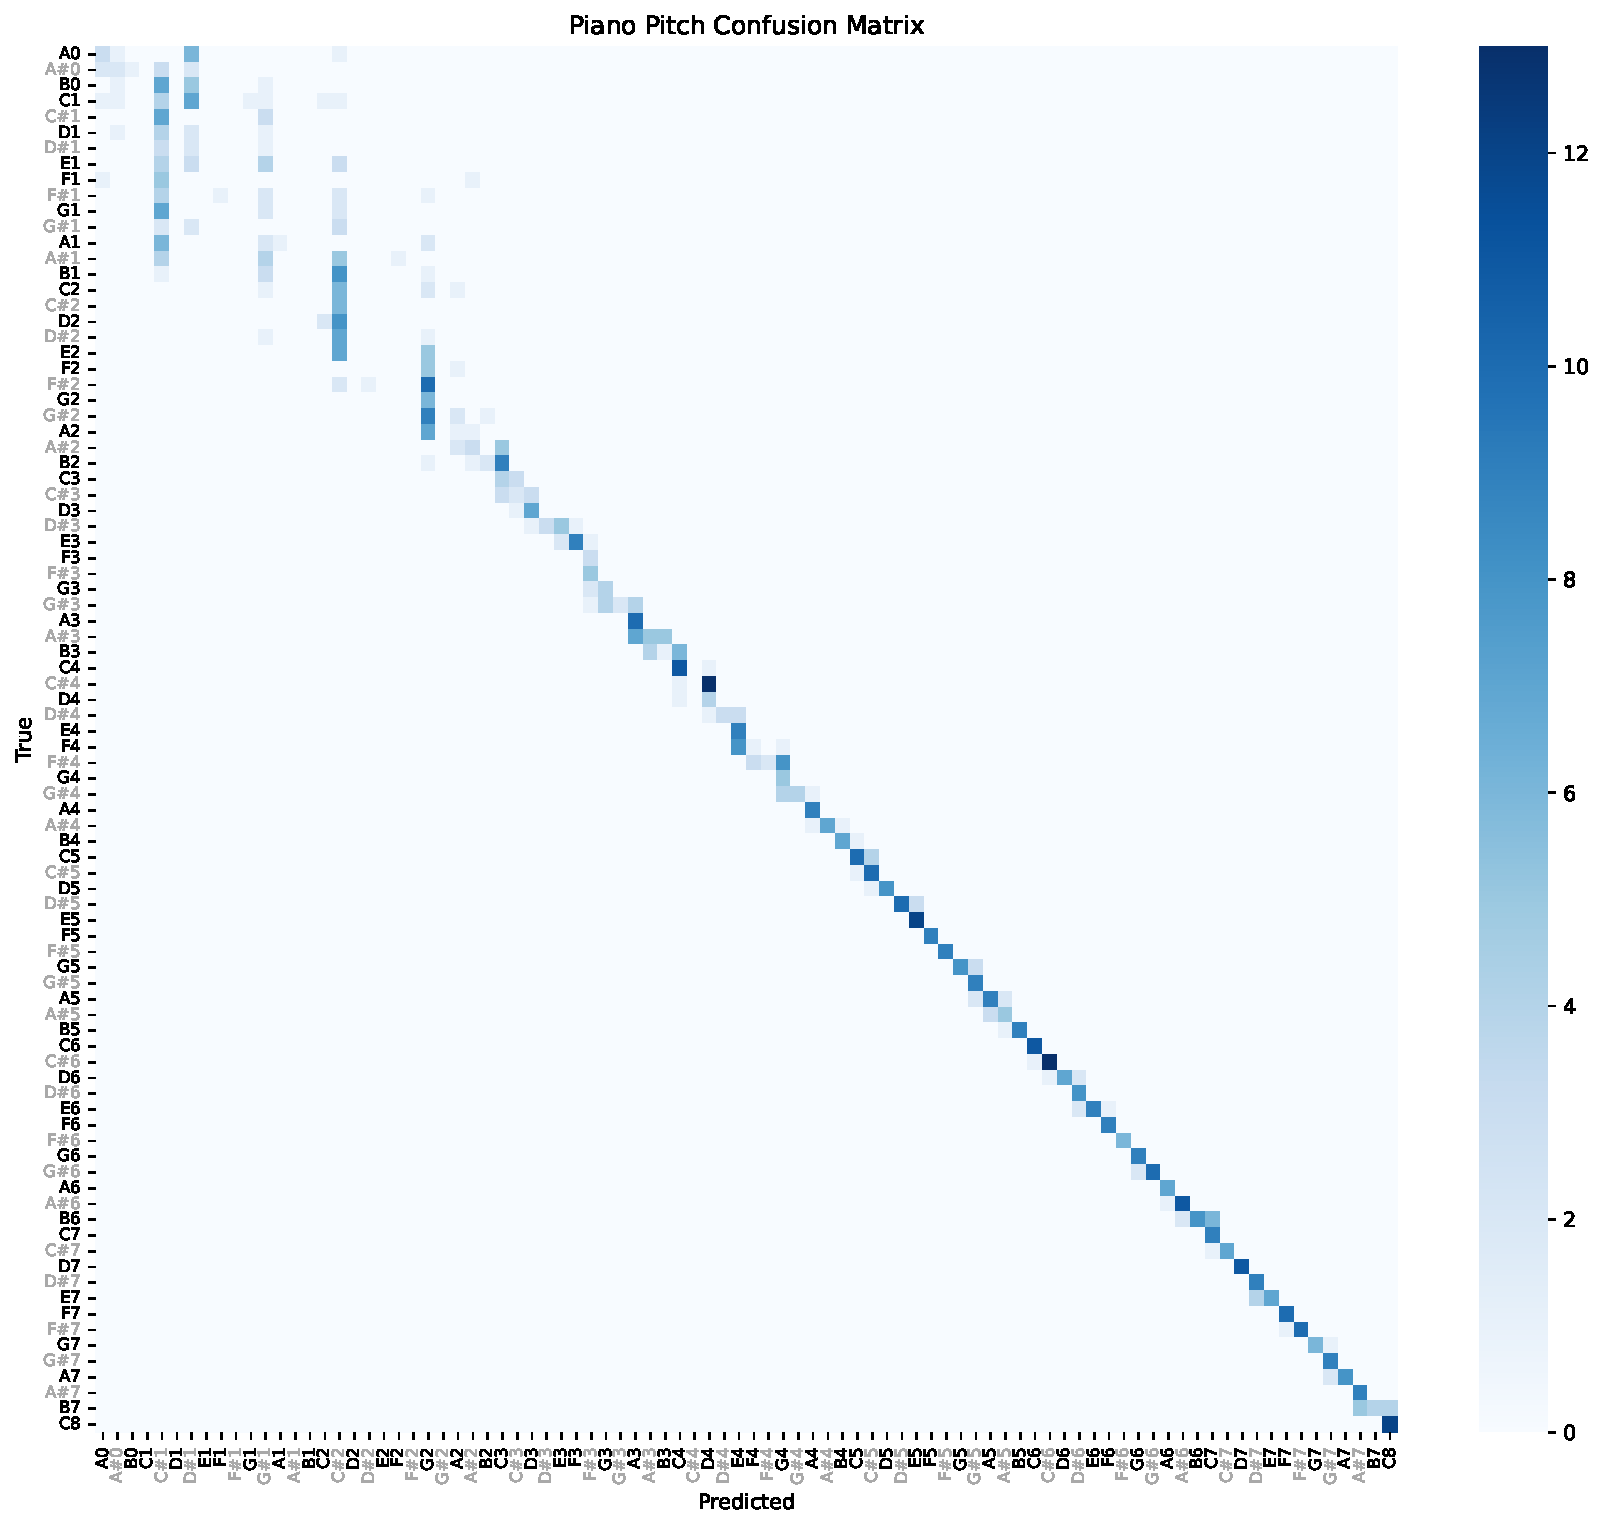
\includegraphics[width=0.85\textwidth]{confusion_piano88_handy.pdf}

\vspace{0.cm}
\small Misclassification starts at B2 (123.47 Hz)
\end{column}
\begin{column}{0.48\textwidth}
\centering
\textbf{Spikify Preprocessing}
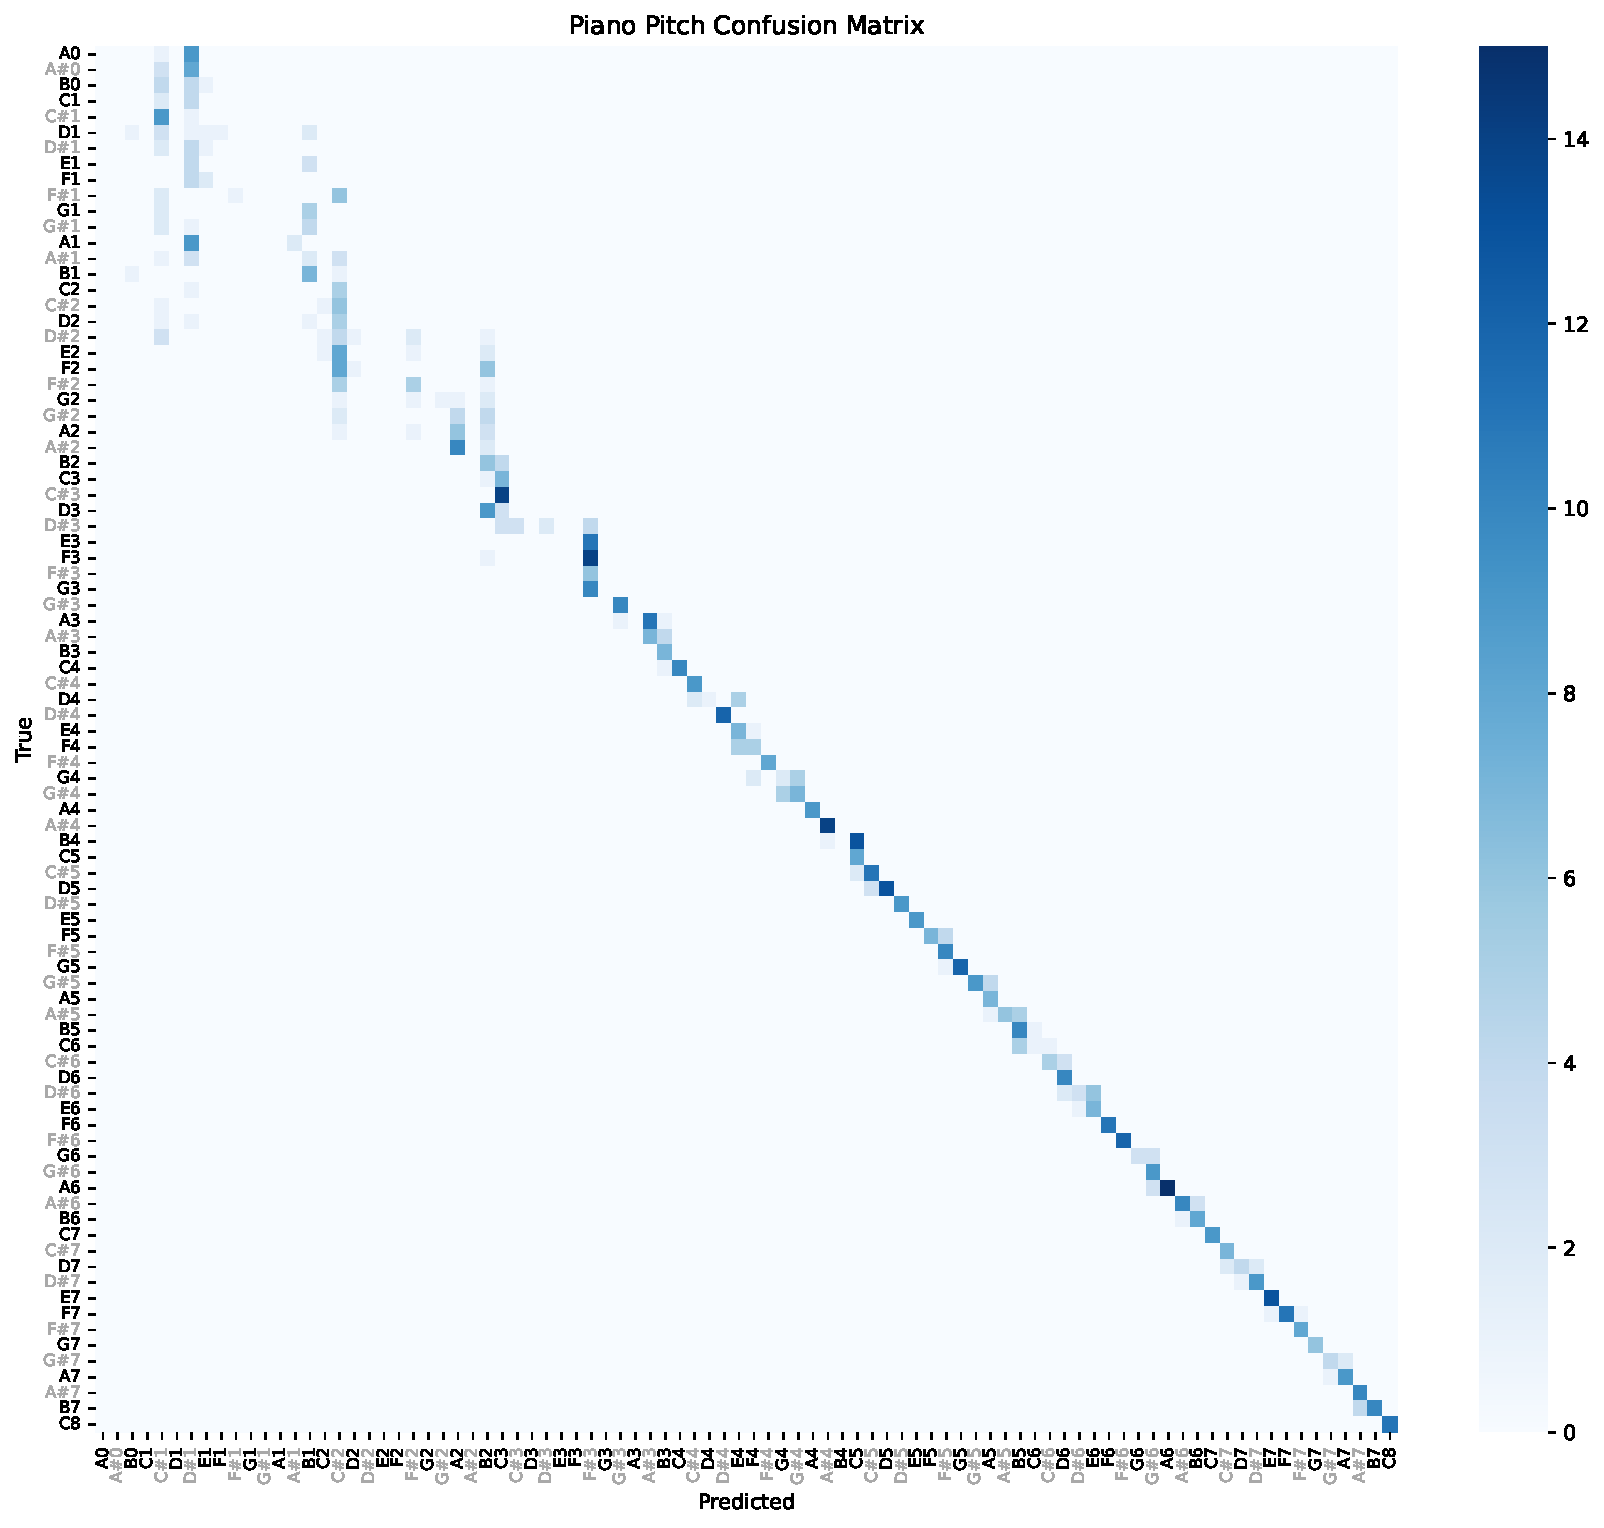
\includegraphics[width=0.85\textwidth]{confusion_piano88_spikify.pdf}

\vspace{0.cm}
\small Misclassification starts at F3 (174.61 Hz)
\end{column}
\end{columns}

\textbf{Key Observation.} \textit{Low-frequency notes are harder to classify.} Handy preprocessing extends accurate classification lower, suggesting better temporal precision at low freqs.

\end{frame}

% =============================================================================
% SECTION 6: EXPERIMENT 3 - STDP UNSUPERVISED LEARNING
% =============================================================================
\section{Experiment 3: STDP Unsupervised Learning}
\begin{frame}{STDP Learning Rule}
	\begin{block}{Classical STDP (Spike-Timing-Dependent Plasticity)}
		\begin{equation}
			\Delta w_{ij} = \begin{cases}
				A_+ e^{-\Delta t/\tau_+} & \text{if } \Delta t = t_j^{\text{post}} - t_i^{\text{pre}} > 0 \quad \text{(LTP)}\\
				-A_- e^{\Delta t/\tau_-} & \text{if } \Delta t < 0 \quad \text{(LTD)}
			\end{cases}
		\end{equation}
	\end{block}
	
	\vspace{-0.3cm}
	\textbf{STDP-WTA Architecture:}
	\begin{itemize}
		\item \textbf{Input:} 50 cochlear channels $\Rightarrow$ \textbf{Output:} 88 LIF neurons (one per piano key) 
		\item \textbf{Winner-Take-All (WTA):} Only highest-spiking neuron updates weights
		\item \textbf{Lateral inhibition:} $I_{\text{inh}} = 0.5 \cdot \sum_{k \neq j} s_k$
	\end{itemize}
	
	\vspace{0.1cm}
	\textbf{Trace-Based Implementation:}
	\begin{equation}
		\text{pre\_trace}(t+1) = \text{pre\_trace}(t) \cdot e^{-1/\tau_{\text{pre}}} + s_i^{\text{pre}}(t)
	\end{equation}
	\begin{equation}
		\Delta w_{ij} = \eta \left( s_j^{\text{post}} \cdot \text{pre\_trace} - s_i^{\text{pre}} \cdot \text{post\_trace} \right)
	\end{equation}
\end{frame}

\begin{frame}{STDP-WTA Architecture}
\begin{center}
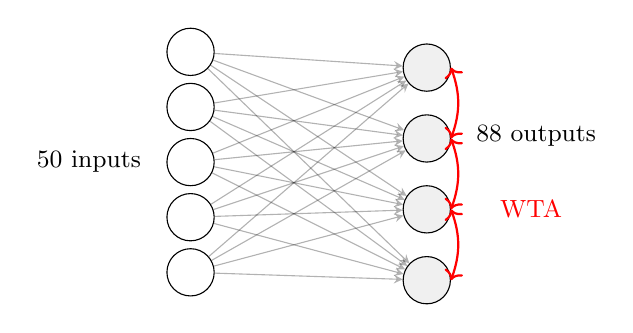
\begin{tikzpicture}[
    node distance=0.8cm,
    input neuron/.style={circle, draw=black, fill=white, minimum size=0.6cm, font=\tiny},
    output neuron/.style={circle, draw=black, fill=headinggrey, minimum size=0.6cm, font=\tiny},
    arrow/.style={->, >=stealth}
]
    % Input layer
    \foreach \i in {1,...,5} {
        \node[input neuron] (in\i) at (0, -\i*0.7) {};
    }
    \node[left=0.2cm of in3] {\small 50 inputs};

    % Output layer (WTA)
    \foreach \o in {1,...,4} {
        \node[output neuron] (out\o) at (3, -\o*0.9) {};
    }
    \node[right=0.2cm of out2.5] {\small 88 outputs};

    % Connections
    \foreach \i in {1,...,5} {
        \foreach \o in {1,...,4} {
            \draw[arrow, opacity=0.3] (in\i) -- (out\o);
        }
    }

    % WTA inhibition
    \draw[thick, <->, red] (out1.east) to[bend left=20] (out2.east);
    \draw[thick, <->, red] (out2.east) to[bend left=20] (out3.east);
    \draw[thick, <->, red] (out3.east) to[bend left=20] (out4.east);
    \node[red, right=0.5cm of out3] {\small WTA};
\end{tikzpicture}
\end{center}

\begin{columns}
	\centering
	\begin{column}{0.48\textwidth}
		\textbf{Trace-Based Implementation:}
		\begin{equation*}
			\text{pre\_trace}(t+1) = \text{pre\_trace}(t) \cdot e^{-1/\tau_{\text{pre}}} + s_i^{\text{pre}}(t)
		\end{equation*}
		\begin{equation*}
			\text{post\_trace}(t+1) = \text{post\_trace}(t) \cdot e^{-1/\tau_{\text{post}}} + s_i^{\text{post}}(t)
		\end{equation*}
		\begin{equation*}
			\Delta w_{ij} = \eta \left( s_j^{\text{post}} \cdot \text{pre\_trace} - s_i^{\text{pre}} \cdot \text{post\_trace} \right)
		\end{equation*}
	\end{column}
	\begin{column}{0.48\textwidth}
		\textbf{Training Procedure:}
		\begin{enumerate}
			\item Forward pass to determine winner (max spike count)
			\item Second pass with STDP update for winner only
			\item Lateral inhibition prevents multiple winners
			\item Homeostatic normalization after each update
		\end{enumerate}
		
		\vspace{0.1cm}
		\textbf{Parameters:} $\tau_{\text{pre}} = \tau_{\text{post}} = 20$ ms, $\eta = 0.002$, $\beta = 0.95$
	\end{column}
\end{columns}

\end{frame}

\begin{frame}{Spike Count Dynamics During Training}
\begin{columns}
\begin{column}{0.48\textwidth}
\centering
\textbf{Handy Preprocessing}
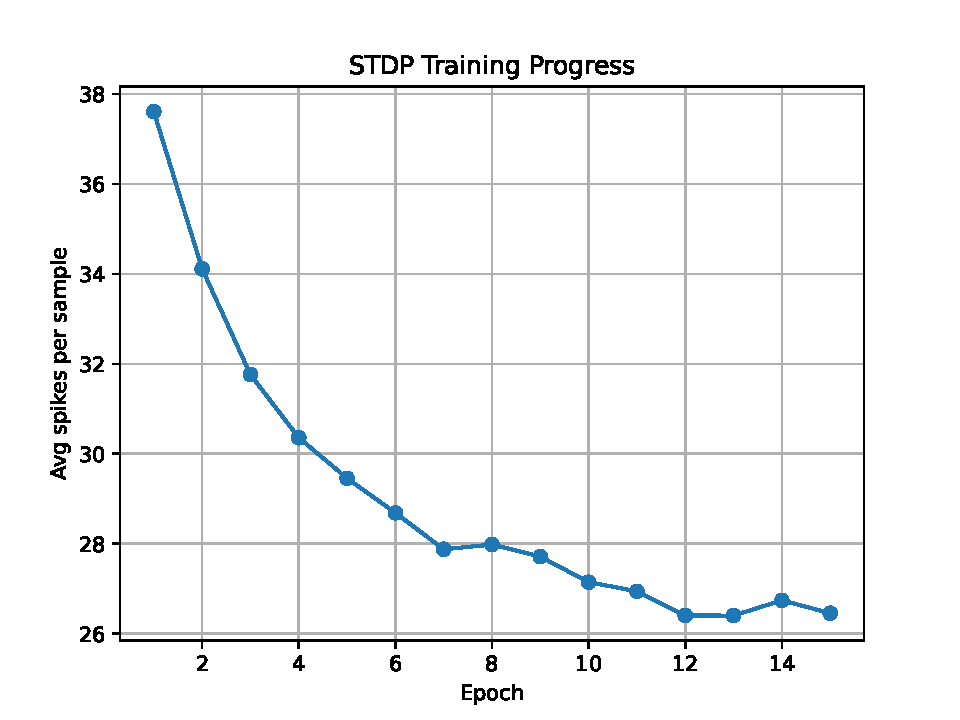
\includegraphics[width=\textwidth]{stdp_spike_count_handy.pdf}

\vspace{0.2cm}
\small Gradual spike count reduction\\indicates stable learning
\end{column}
\begin{column}{0.48\textwidth}
\centering
\textbf{Spikify Preprocessing}
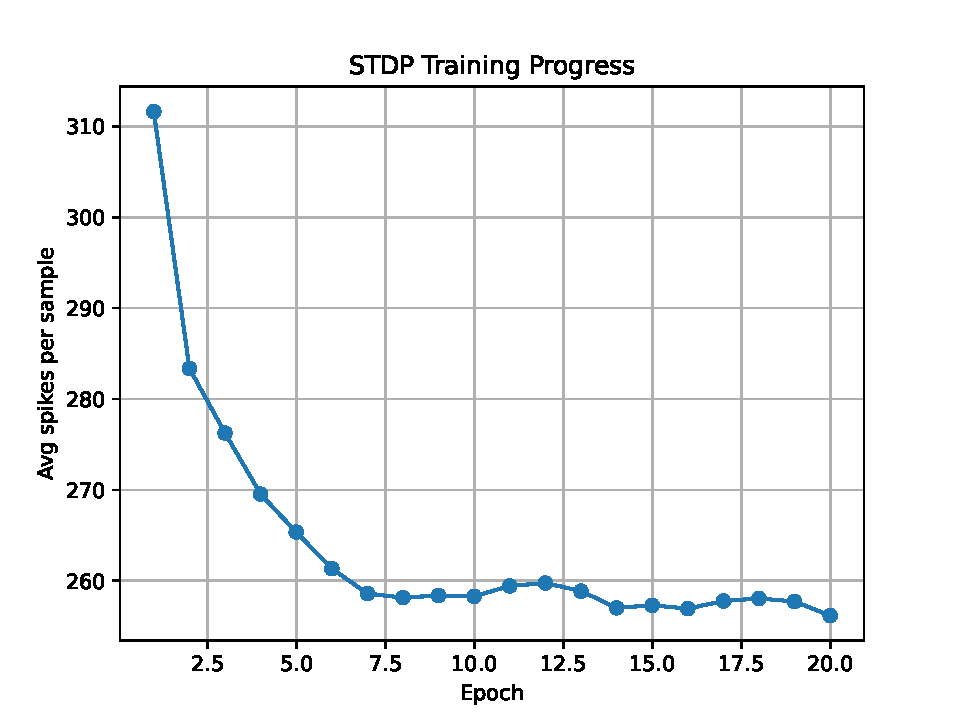
\includegraphics[width=\textwidth]{stdp_spike_count_spikify.pdf}

\vspace{0.2cm}
\small Higher variance in spike counts\\more unstable dynamics
\end{column}
\end{columns}
\end{frame}

\begin{frame}{STDP Confusion Matrices: Learning Quality}
\begin{columns}
\begin{column}{0.48\textwidth}
\centering
\textbf{Handy Preprocessing}
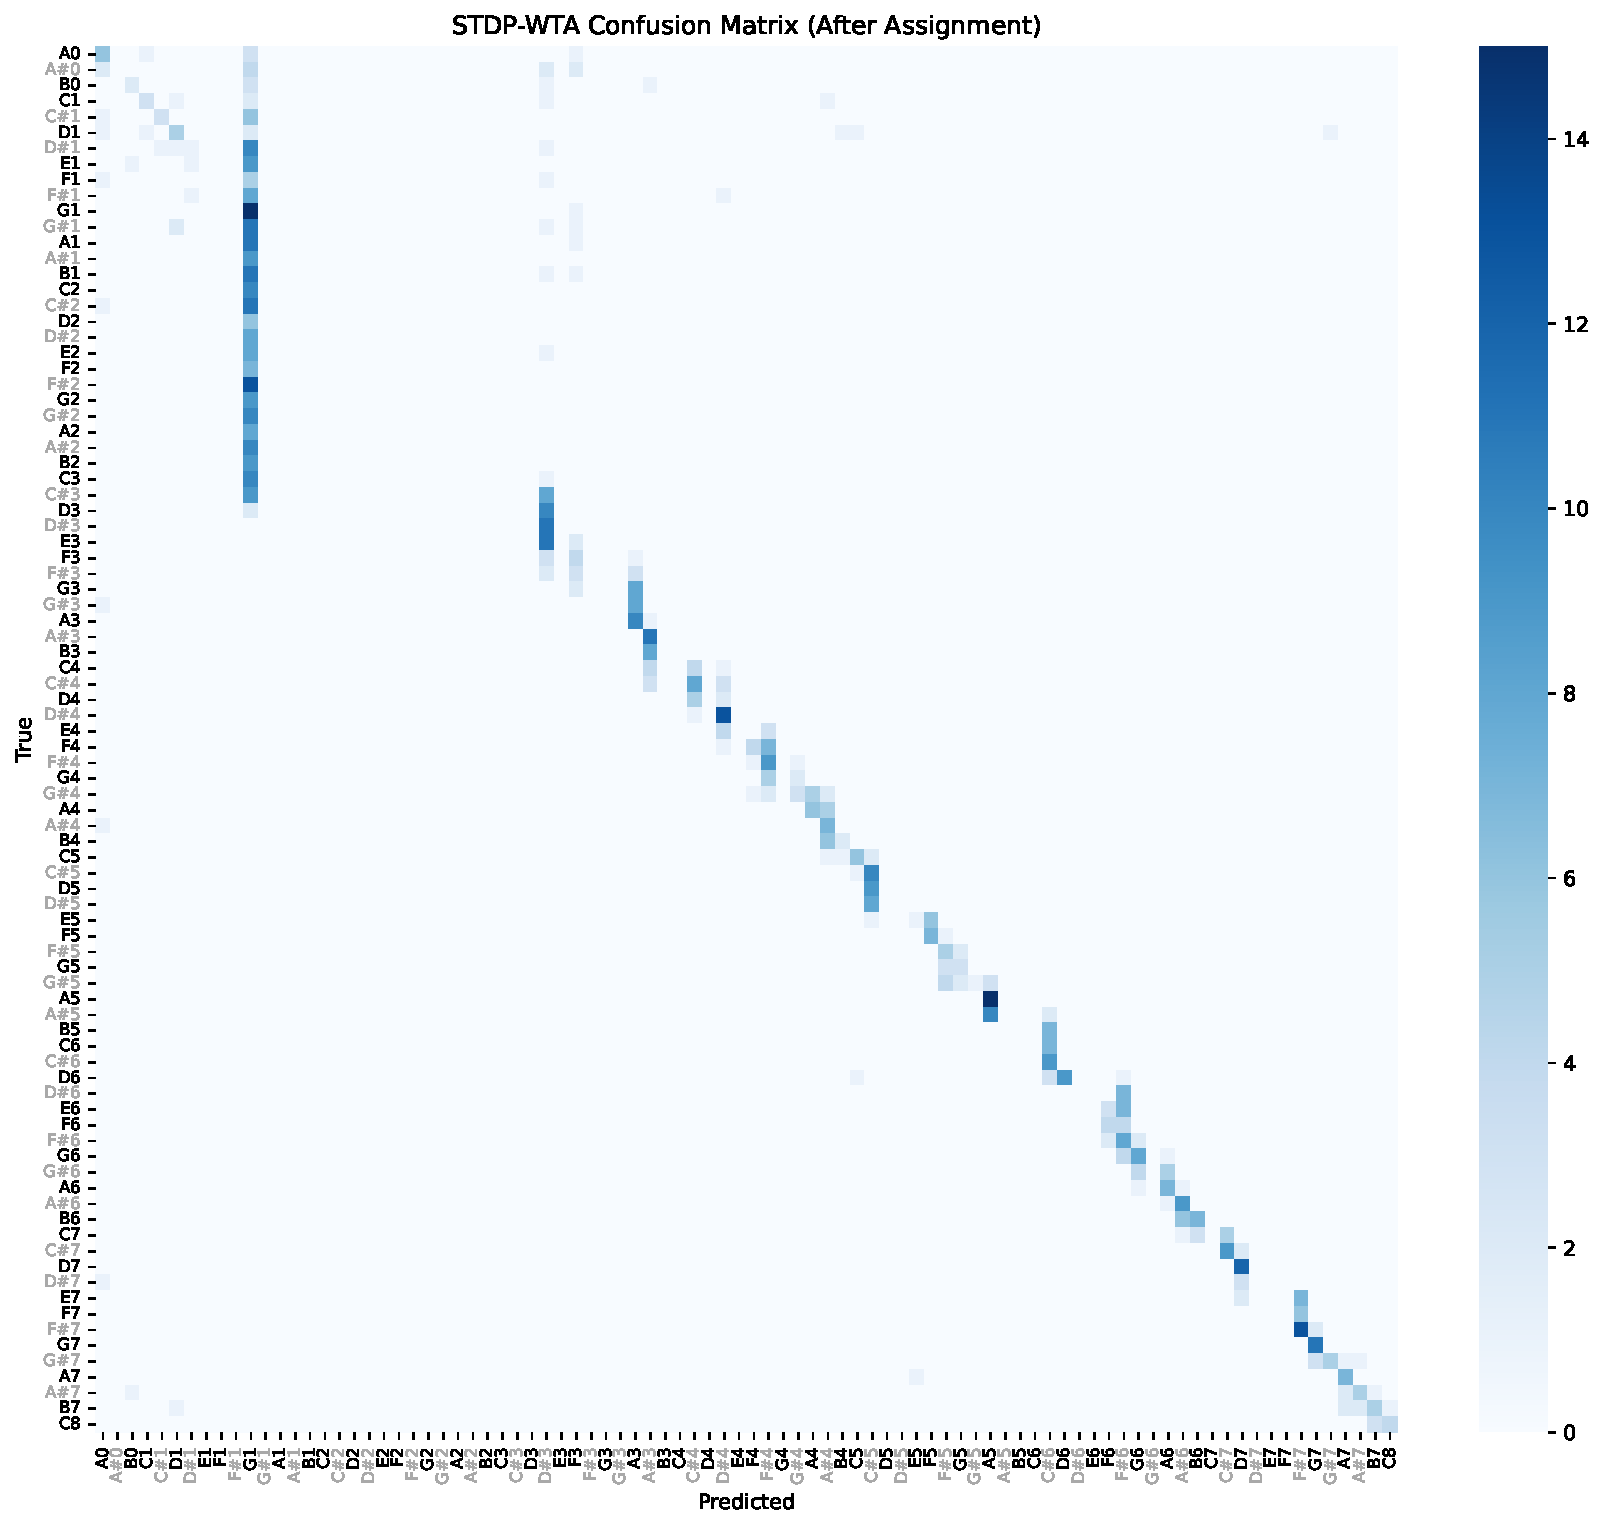
\includegraphics[width=0.85\textwidth]{confusion_stdp_handy.pdf}

\vspace{0.2cm}
\small Misclassifications (E3 and below)\\concentrated on G1/A1
\end{column}
\begin{column}{0.48\textwidth}
\centering
\textbf{Spikify Preprocessing}
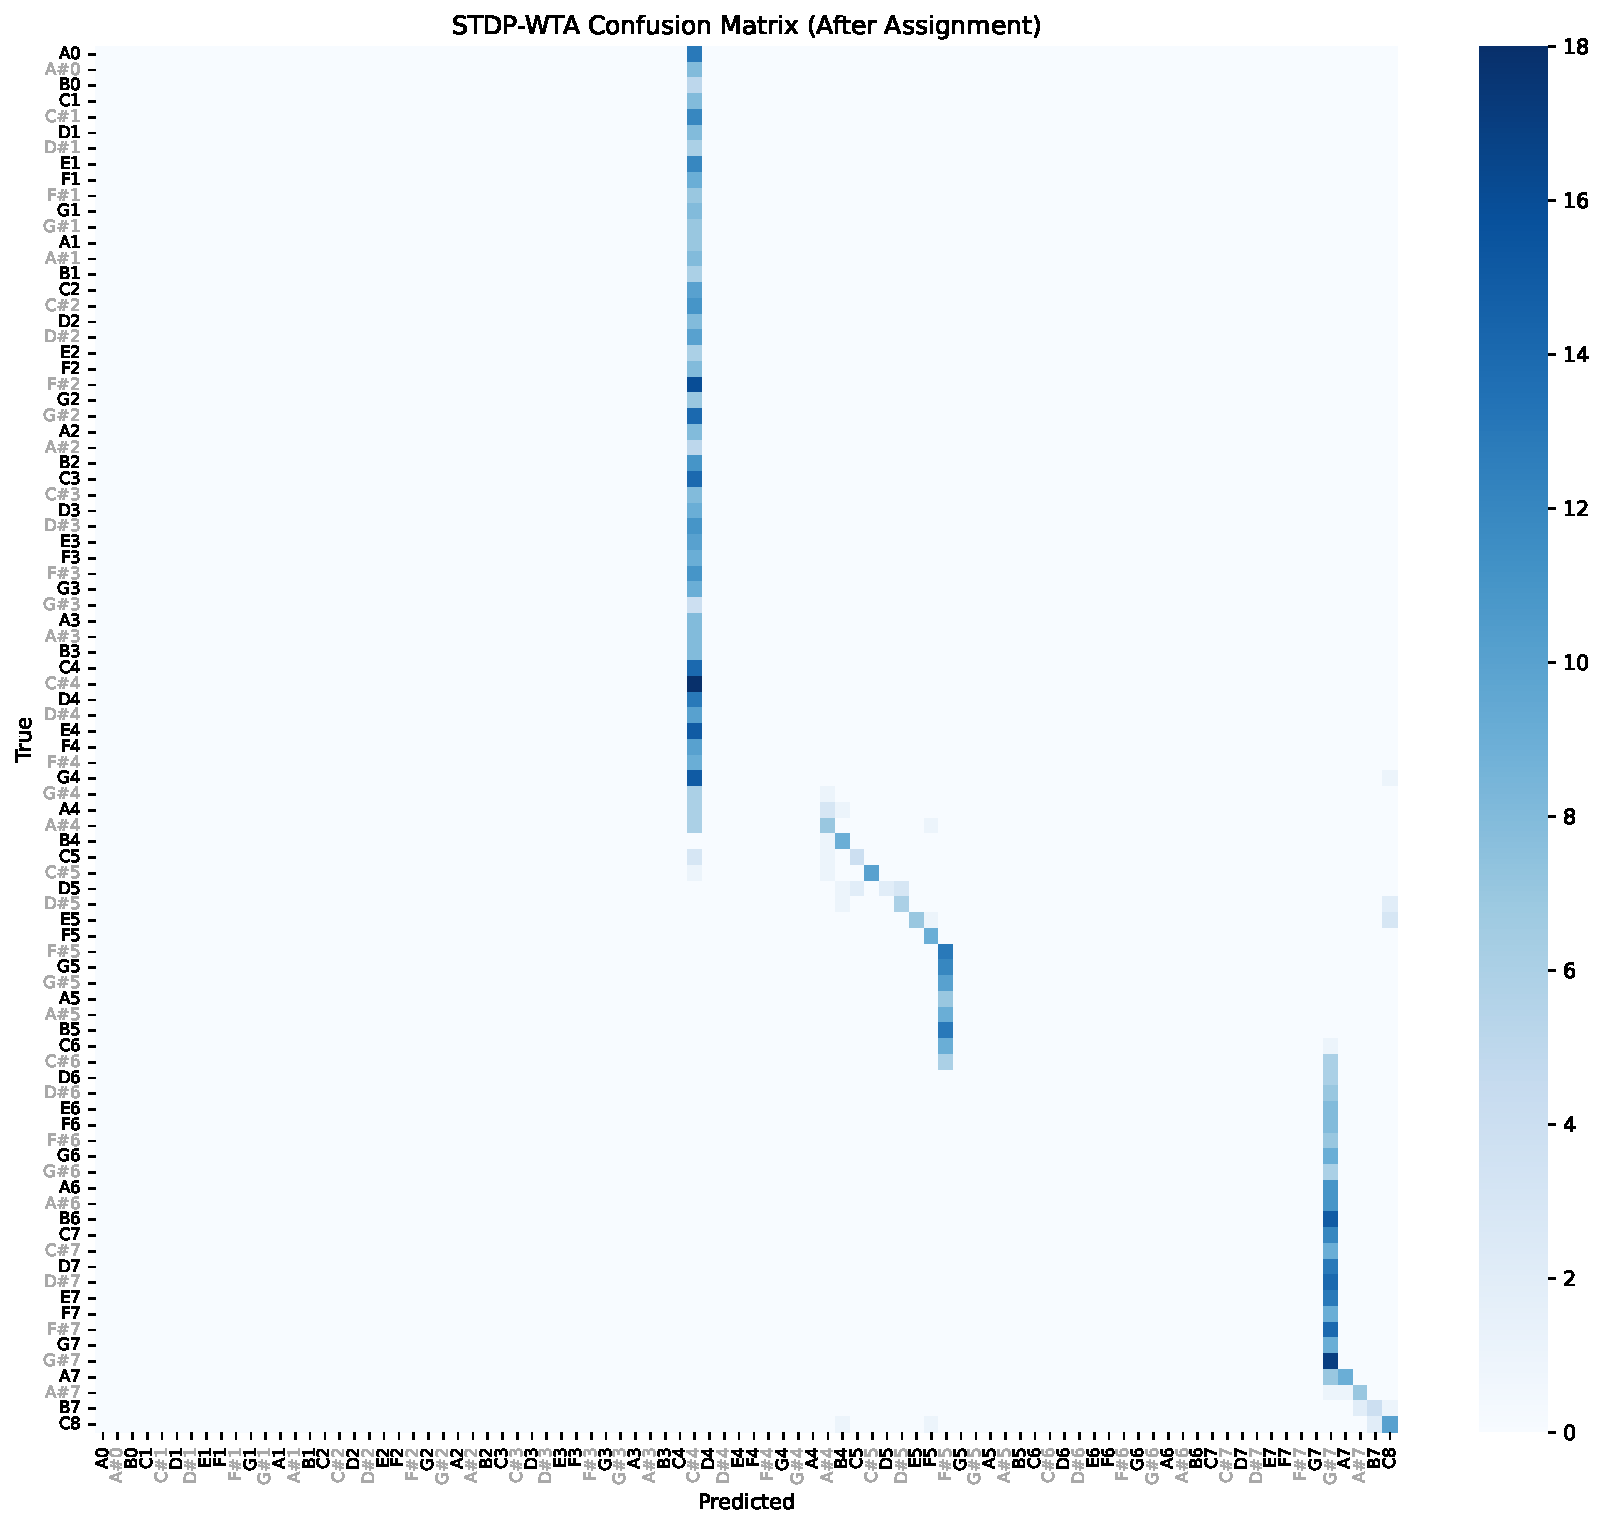
\includegraphics[width=0.85\textwidth]{confusion_stdp_spikify.pdf}

\vspace{0.2cm}
\small Diffuse misclassifications\\across frequency range
\end{column}
\end{columns}
\end{frame}

% =============================================================================
% SECTION 7: KEY FINDINGS SUMMARY
% =============================================================================
\section{Key Findings Summary}

\begin{frame}{Comparison: Handy vs Spikify}
\begin{center}
\begin{tabular}{lcc}
\toprule
\textbf{Property} & \textbf{Handy} & \textbf{Spikify} \\
\midrule
Training speed & Slower & \textbf{Faster} \\
Noise robustness & \textbf{High} (stable) & Low (unstable) \\
Low-frequency accuracy & \textbf{B2 and above} & F3 and above \\
STDP convergence & \textbf{Stable} & Fluctuating \\
Error pattern & \textbf{Structured} (octave) & Diffuse \\
Temporal precision & \textbf{Better} phase-locking & Standard \\
\bottomrule
\end{tabular}
\end{center}

\vspace{0.4cm}
\textbf{Hypothesis:} Handy's relative thresholding and global normalization preserve temporal structure better, enabling more robust phase-locking to stimulus frequency---critical for noise immunity.

\vspace{0.3cm}
\textbf{Trade-off:} Spikify's optimized implementation prioritizes training efficiency over noise robustness.
\end{frame}


\section{Toward ``Absolute Pitch'' Model}

\begin{frame}{Conclusions. Current Limitation and Biological Inspiration}
\begin{block}{Current Approach Limitation}
Training on all 88 keys simultaneously requires the model to learn:\
\begin{enumerate}
    \item Absolute frequency discrimination (within-octave)
    \item Octave equivalence (C4 vs C5)
    \item Full harmonic structure across 7+ octaves
\end{enumerate}
\textit{This is computationally expensive. Possibly biologically implausible?}
\end{block}

\vspace{0.1cm}
\textbf{Human Absolute Pitch Development:}
\begin{itemize}
    \item Early childhood exposure to pitch-class associations
    \item Learning within limited frequency range initially
    \item Generalization to full frequency range later
    \item Octave equivalence emerges from harmonic structure
\end{itemize}

\vspace{0.1cm}
\textbf{Future Research:} Train on single octave (12 notes), then test generalization.
\end{frame}

\begin{frame}{Proposed ``Absolute Pitch'' Architecture}
\begin{columns}
	\centering
	\begin{column}{0.48\textwidth}
		\textbf{1. Single-Octave Training (C4--B4)}
		\begin{itemize}
			\item 12 classes instead of 88
			\item Learn pitch-class representation
			\item Octave-invariant feature extraction
		\end{itemize}
	\end{column}
	\begin{column}{0.48\textwidth}
		\textbf{2. Octave Generalization}
		\begin{itemize}
			\item Transfer learned pitch-class representations
			\item Add octave detection layer
			\item Fine-tune on full range
		\end{itemize}
	\end{column}
\end{columns}




\vspace{0.3cm}
\textbf{Octave-Invariant Features:}
\begin{equation}
f_{\text{normalized}} = f / 2^{\lfloor\log_2(f/f_{\text{ref}})\rfloor}
\end{equation}

\vspace{0.2cm}
\textbf{Potential Benefits:}
\begin{itemize}
    \item Reduced parameter space (12 vs 88 output neurons)
    \item Better generalization through octave equivalence
    \item More biologically plausible learning trajectory?
\end{itemize}
\end{frame}

% =============================================================================
% SECTION 9: CONCLUSIONS
% =============================================================================
\section{Conclusions}

\begin{frame}{Summary of Contributions}
\begin{enumerate}
    \item \textbf{Preprocessing Pipeline:}
    \begin{itemize}
        \item Implemented custom ERB scales (Linear, Quadratic, Voicebox)
        \item Discovered and fixed critical scaling bug
        \item Established relative-threshold Poisson encoding
    \end{itemize}

    \item \textbf{3-Tone Classification:}
    \begin{itemize}
        \item Achieved 100\% accuracy after preprocessing fix
        \item Demonstrated superior noise robustness of handy preprocessing
    \end{itemize}

    \item \textbf{88-Key Piano Classification:}
    \begin{itemize}
        \item 58\% accuracy on full piano range
        \item Identified low-frequency classification challenges
    \end{itemize}

    \item \textbf{STDP Unsupervised Learning:}
    \begin{itemize}
        \item Implemented competitive WTA learning
        \item Showed structured learning with handy preprocessing
    \end{itemize}
\end{enumerate}
\end{frame}

\begin{frame}{Future Directions}
\textbf{Immediate Improvements:}
\begin{itemize}
    \item Implement ``absolute pitch'' model with octave training
\end{itemize}

\vspace{0.3cm}
\textbf{Research Questions:}
\begin{itemize}
    \item Can octave-invariant features improve generalization?
    \item How does filterbank density affect low-frequency performance?
    \item Can STDP with structured inhibition improve note separation?
\end{itemize}

\vspace{0.3cm}
\textbf{Biological Extensions:}
\begin{itemize}
    \item Model binaural cues for pitch in noise
    \item Explore place-temporal coding trade-offs
\end{itemize}
\end{frame}

% =============================================================================
% REFERENCES
% =============================================================================
\section*{References}

\begin{frame}[noframenumbering, plain]{References} 
\footnotesize
\begin{enumerate}
    \item Pan, Z., et al. (2019). An efficient and perceptually motivated auditory neural encoding algorithm for SNNs. \textit{IEEE TNNLS}.

    \item Song, Z., et al. (2024). Spiking-LEAF: A Learnable Auditory front-end for Spiking Neural Networks. \textit{IEEE TPAMI}.

    \item Wu, J., et al. (2018). A spiking neural network framework for robust sound classification. \textit{Frontiers in Neuroscience}.

    \item Alsakkal, M.H., \& Wijekoon, J. (2025). Spiketrum: An FPGA-based implementation of a neuromorphic cochlea. \textit{IEEE TCAS}.

    \item Saddler, M.R., et al. (2021). Deep neural network models reveal interplay of peripheral coding and stimulus statistics in pitch perception. \textit{Nature Communications}.

    \item Glasberg, B.R., \& Moore, B.C.J. (1990). Derivation of auditory filter shapes from notched-noise data. \textit{Hearing Research}.

    \item Cariani, P. (1999). Temporal coding of periodicity pitch in the auditory system. \textit{Neural Plasticity}.
\end{enumerate}
\end{frame}

% =============================================================================
% END
% =============================================================================
{
\setbeamertemplate{frametitle}{}
\begin{frame}[noframenumbering, plain] 
\vspace{2cm}
\begin{center}
    {\Large\textbf{Thank You For Your Attention!}}\\[1cm]
    %{\normalsize Questions?}\\[1.5cm]
    {\small Neuromorphic Computing Course Project}\\
    {\small Skoltech, May 2026}
\end{center}
\end{frame}
}

\end{document}
